% ====================================================================
% graphite_ica_ch1_v7-04b.tex — Chapter 1 (v7-04 의 미세 보완본; v7-04.tex 원본 보존)
%   흑연 음극 dQ/dV(ICA) 이론 — v11_final.py 의 클래스 계산 진행(N0->N9)을 절 순서로,
%   그 순서를 이해하는 데 필요한 물리식만 그 순서대로 유도한다.
%   형식 = v5(graphite_ica_ch1_Opus_v5.tex) 계열(수식 주도). 식별자·기호·부호는 v11_final 과 1:1.
%   그림은 전부 신규 TikZ(내부 텍스트 영어 ASCII). build: xelatex 2-pass.
%   [v7-04 -> v7-04b 보완] w^eff 게이트(tr.get('w') is None) 가 GRAPHITE_STAGING_LIT 의
%     'w' 키 때문에 막혀 use_w_eff=True 라도 실효 없음을 본문·표·코드박스에 명시(§1.5/N0표/§1.9).
%     그 외 통독 중 미세 다리·표기 다듬기. 부호 8/8·식 사슬·환원 검산 불변(보완이 무결 깨지 않음).
% ====================================================================
\documentclass[11pt,a4paper]{article}
\usepackage[margin=22mm]{geometry}
\usepackage{kotex}
\setmonofont{D2Coding}[Scale=MatchLowercase]
\usepackage{amsmath,amssymb,mathtools,bm}
\usepackage{booktabs,longtable,array}
\usepackage{enumitem}
\usepackage{amsthm}
\usepackage{hyperref}
\usepackage{fancyhdr}
\usepackage{lastpage}
\usepackage{setspace}
\usepackage{tikz}
\usetikzlibrary{positioning,calc}
\setstretch{1.12}
\setlength{\parskip}{0.45em}\setlength{\parindent}{0pt}\setlength{\headheight}{14pt}
\setlength{\emergencystretch}{2em}
\hypersetup{colorlinks=true, linkcolor=blue, urlcolor=blue, citecolor=blue,
  pdftitle={흑연 음극 dQ/dV 이론: 코드 진행 어레인지 — Chapter 1 (v7-04b)}}
\pagestyle{fancy}\fancyhf{}
\lhead{흑연 음극 $dQ/dV$ 이론 — Ch.1 (v7, 코드-진행 어레인지)}\rhead{\thepage/\pageref{LastPage}}
\renewcommand{\headrulewidth}{0.4pt}

\newtheorem*{keybox}{핵심}
\newtheorem*{codebox}{코드 대응}
\newtheorem*{boundbox}{유효 범위}
\newtheorem*{verifybox}{검산}

\newcommand{\dd}{\mathrm{d}}
\newcommand{\eff}{\mathrm{eff}}
\newcommand{\eq}{\mathrm{eq}}
\newcommand{\app}{\mathrm{app}}
\newcommand{\cell}{\mathrm{cell}}
\newcommand{\bg}{\mathrm{bg}}
\newcommand{\work}{\mathrm{work}}
\newcommand{\rep}{\mathrm{rep}}
\newcommand{\hys}{\mathrm{hys}}
\newcommand{\lagg}{\mathrm{lag}}
\newcommand{\dis}{\mathrm{dis}}
\newcommand{\chg}{\mathrm{chg}}
\newcommand{\sgn}{\sigma_d}

\renewcommand{\theequation}{1.\arabic{equation}}
\renewcommand{\thesection}{1.\arabic{section}}
\title{\textbf{\LARGE Chapter 1}\\[0.35em]\Large 흑연 음극 $dQ/dV$ 이론: 한 곡선을 그리는 계산 진행과 그 물리 — 코드-진행판}
\author{}
\date{}

% TOC: widen number boxes
\makeatletter
\renewcommand*\l@section[2]{%
  \ifnum \c@tocdepth >\z@
    \addpenalty\@secpenalty
    \addvspace{1.0em \@plus\p@}%
    \setlength\@tempdima{2.3em}%
    \begingroup
      \parindent \z@ \rightskip \@pnumwidth
      \parfillskip -\@pnumwidth
      \leavevmode \bfseries
      \advance\leftskip\@tempdima
      \hskip -\leftskip
      #1\nobreak\hfil
      \nobreak\hb@xt@\@pnumwidth{\hss #2\kern-\p@\kern\p@}\par
    \endgroup
  \fi}
\renewcommand*\l@subsection{\@dottedtocline{2}{2.3em}{3.2em}}
\makeatother

\begin{document}
\maketitle

% ====================================================================
\section*{서론 — 코드가 한 곡선을 그리는 순서가 본 장의 차례다}
\addcontentsline{toc}{section}{서론}
% ====================================================================
리튬이온전지 흑연 음극의 incremental capacity analysis(ICA)는 충방전 곡선 $Q(V)$ 의 미분 $\dd Q/\dd V$ 를 본다. 흑연은 staging 상전이(stage $4\!\to\!3\!\to\!2\mathrm L\!\to\!2\!\to\!1$)를 거치며 각 전이 전위에서 두 상이 공존하면 전위가 거의 평탄해 좁은 $\dd V$ 에 큰 $\dd Q$ 가 몰려 $\dd Q/\dd V$ 가 치솟는다. 이 peak 의 위치$\cdot$너비$\cdot$높이가 온도$\cdot$전위$\cdot$C-rate 세 인자에 따라 변하는 방식이 본 장의 대상이다.

본 장은 한 가지 점에서 일반 이론 서술과 다르다 — \textbf{서술 순서를 구현 코드가 한 곡선을 그리는 계산 진행에 맞춘다}. 구현(\texttt{GraphiteAnodeDischargeDQDV} 클래스)은 실험조건 $(\text{direction},\,c\text{-rate},\,T,\,Q_\cell)$ 을 받아 메서드 \texttt{curve}$\to$\texttt{dqdv} 로 한 $\dd Q/\dd V$ 곡선을 반환한다. 그 계산은 다음 순서로 진행한다:
\begin{enumerate}[label=\textbf{N\arabic*.},start=0,leftmargin=2.6em,itemsep=1pt]
\item 실험조건을 모델 입력 $\sgn,\,|I|,\,T,\,Q_\cell$ 로 환산(\S\ref{sec:setup}).
\item 분극 — 측정 전위에서 IR 분극을 벗겨 내부 전위 $V_n=V_\app-\sgn|I|R_n$ 으로(\S\ref{sec:pol}).
\item 평형 중심 $U_j(T)=(-\Delta H_{\mathrm{rxn}}+T\Delta S_{\mathrm{rxn}})/F$(\S\ref{sec:Uj}).
\item 히스테리시스 분기 중심 $U_j^d=U_j+\tfrac12\sgn h_\eta\gamma\,\Delta U^\hys$(\S\ref{sec:hys}).
\item 폭 $w=nRT/F$ 와 평형 점유 $\xi_\eq=\mathrm{logistic}[\sgn(V_\work-U_j^d)/w]$(\S\ref{sec:width}).
\item 평형 peak $Q_j\xi_\eq(1-\xi_\eq)/w$($|I|\to0$ 한계, \S\ref{sec:eqpeak}).
\item 동역학 지연 길이 $L_V$ — 컷 affinity$\cdot$방향별 $\chi_d$$\cdot$유효 장벽 $\Delta H_a^\eff$ 에서(\S\ref{sec:lag}).
\item 인과 기억 꼬리 — 지수 저역통과, 충전 격자 역전(\S\ref{sec:tail}).
\item 합산 $\dd Q/\dd V=C_\bg+\sum_jQ_j[\text{평형}-\text{지연}]$, staging 4전이(\S\ref{sec:sum}).
\end{enumerate}
각 절은 그 단계의 곡선을 만드는 데 \emph{필요한 물리식만} 그 자리에서 유도한다. 곡선에 쓰이지 않는 일반론은 결과식이 뒤 절에 물리는 한에서만 인용한다. 주 전개는 방전($\sgn=+1$)이고, 충방전 히스테리시스와 충전 꼬리 역전은 같은 식의 $\sgn$ 분기로 흡수한다(N3$\cdot$N8). 흑연 staging 의 갤러리 채움을 그림~\ref{fig:staging} 에 둔다 — 각 stage 전이가 $\dd Q/\dd V$ 에 peak 하나를 남기고, 본 장의 합산(N9)이 이 네 전이를 더한다.

\begin{figure}[t]
\centering
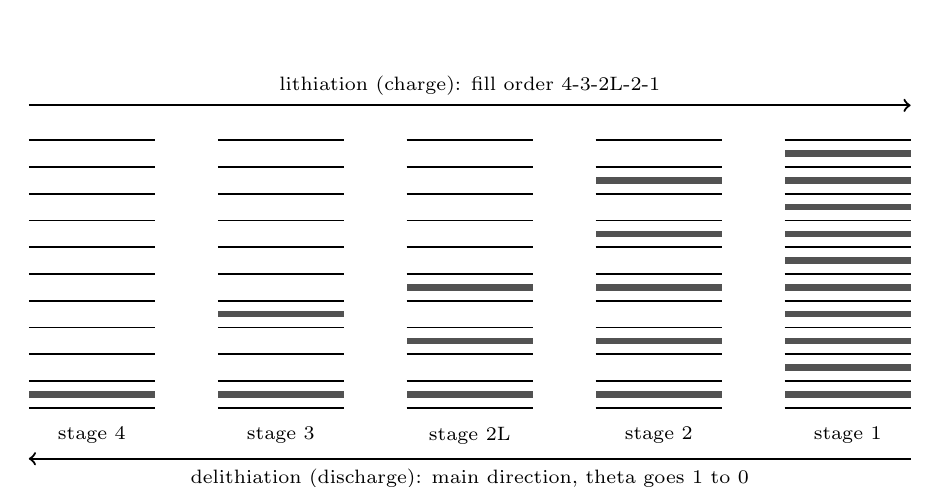
\begin{tikzpicture}[x=1.0cm,y=0.34cm]
% four stage columns: occupancy stripes get denser toward stage 1 (LiC6).
% Each column = graphene sheets (lines) with intercalated-Li bands (filled).
\foreach \cx/\lab/\fillrows in {%
  0/{stage 4}/{1},%
  2.4/{stage 3}/{1,4},%
  4.8/{stage 2L}/{1,3,5},%
  7.2/{stage 2}/{1,3,5,7,9},%
  9.6/{stage 1}/{1,2,3,4,5,6,7,8,9,10}}{
  \foreach \r in {0,1,2,3,4,5,6,7,8,9,10}{
    \draw[semithick] (\cx,\r) -- (\cx+1.6,\r);
  }
  \foreach \fr in \fillrows{
    \fill[black!68] (\cx,{\fr-0.62}) rectangle (\cx+1.6,{\fr-0.38});
  }
  \node[below,font=\scriptsize] at (\cx+0.8,-0.35) {\lab};
}
\draw[->,thick] (0,11.3) -- (11.2,11.3) node[pos=0.5,above,font=\scriptsize] {lithiation (charge): fill order 4-3-2L-2-1};
\draw[<-,thick] (0,-1.9) -- (11.2,-1.9) node[pos=0.5,below,font=\scriptsize] {delithiation (discharge): main direction, theta goes 1 to 0};
\end{tikzpicture}
\caption{흑연 staging 의 갤러리 채움 도식(신규 작성). 수평선이 그래핀 층, 검은 띠가 리튬이 든 층간 갤러리다. 오른쪽으로 갈수록 채움이 조밀해져 stage 1($\mathrm{LiC_6}$, 완전 채움)에 닿고, 각 stage 전이가 $\dd Q/\dd V$ 에 peak 하나를 남긴다. 코드의 \texttt{GRAPHITE\_STAGING\_LIT} 네 전이가 이 네 갈래 채움에 대응한다(\S\ref{sec:sum}). 위 화살표가 리튬화(충전), 아래가 탈리튬화(방전, 본 장의 주 방향).}
\label{fig:staging}
\end{figure}

\tableofcontents
\newpage

% ====================================================================
\section{기호와 실험조건 매핑 (N0)}\label{sec:setup}
% ====================================================================
계산의 첫 단계는 실험조건을 모델 입력으로 환산하는 것이다 — 그 입력이 이후 모든 식의 인자가 되므로 먼저 둔다. 표는 본 장 전개 순서(N0$\to$N9)대로 배열한 사전이고, 코드 식별자를 함께 적는다.

\textbf{전이 인덱스.} $j=1,\dots,N_p$($N_p=4$, staging 4전이). 전이 $j$ 마다 점유율 $\theta_j$, 진행률 $\xi_j\equiv1-\theta_j$(방전 시 $\theta_j:1\to0$, $\xi_j:0\to1$).

\textbf{부호 규약(★최우선).} 방향 부호 $\sgn\in\{+1,-1\}$, 방전 $+1$$\cdot$충전 $-1$. 코드 \texttt{curve} 가 문자열/정수 \texttt{direction} 을 \texttt{\_direction\_to\_sigma} 로 환산한다. $\sgn$ 의 작용처는 셋뿐이다 — \textbf{분극 부호}(N1)$\cdot$\textbf{분기 중심 선택}(N3)$\cdot$\textbf{꼬리 인과 방향}(N8). 평형 종 자체(N5$\cdot$N6)는 logistic 인자 안 $\sgn$ 으로 들어가되 peak 부호는 방향 불변이다(N6 에서 보인다). 본 장 전반의 단일 사슬 — 방전 시 $V$ 증가 $\Rightarrow$ 탈리튬화 진행 $\xi$ 증가, 충전 $\dd Q/\dd V$ 는 방전의 거울(부호 양수 유지) — 에 모든 절이 정합해야 한다.

\begin{longtable}{p{0.15\textwidth} p{0.20\textwidth} p{0.57\textwidth}}
\toprule 기호 & 코드 식별자 & 의미 / 단위 \\ \midrule \endhead
\multicolumn{3}{l}{\emph{— 실험조건과 입력(N0$\cdot$N1) —}}\\
$\sgn$ & \texttt{s},\,\texttt{sigma\_d} & 방향 부호 $+1$ 방전 / $-1$ 충전 \\
$|I|$ & \texttt{I\_abs} & 전류 크기 [A] $=c\text{-rate}\cdot Q_\cell$($\ge0$) \\
$c\text{-rate}$ & \texttt{c\_rate} & 충방전 율 [1/s] ($Q_\cell$ 가 [C] 라 $|I|=c\text{-rate}\cdot Q_\cell$ 가 [A]) \\
$T$ & \texttt{T} & 온도 [K] (스칼라 등온, 또는 $V_\app$ 길이 배열 $T(V)$) \\
$Q_\cell$ & \texttt{Q\_cell} & 셀 용량(전하) [C]$=$[A$\cdot$s]; $q=Q/Q_\cell$ 무차원 sto 축($>0$) \\
$R_n$ & \texttt{Rn} & 직렬 분극 저항 [$\Omega$] \\
$V_\app,\,V_n$ & \texttt{V\_app},\,\texttt{V\_n} & 인가(측정) 전위 / 내부 전위 [V] \\
$V_\work$ & \texttt{V\_work} & 작업 격자 전위 [V](꼬리 여유 pad 포함) \\
$C_\bg$ & \texttt{Cbg} & 배경 미분용량 [C/V] (상수 또는 $V$ 함수) \\
\multicolumn{3}{l}{\emph{— 평형 중심$\cdot$폭$\cdot$점유(N2$\cdot$N4$\cdot$N5$\cdot$N6) —}}\\
$U_j$ & \texttt{U},\,\texttt{func\_U\_j} & 평형 중심 전위 [V] (또는 $\Delta H_{\mathrm{rxn}},\Delta S_{\mathrm{rxn}}$ 환산) \\
$\Delta H_{\mathrm{rxn}},\Delta S_{\mathrm{rxn}}$ & \texttt{dH\_rxn},\,\texttt{dS\_rxn} & 삽입 반응 엔탈피$\cdot$엔트로피 [J/mol]$\cdot$[J/mol/K] \\
$n$ & \texttt{n} & 폭 다중도(없으면 1) \\
$w$ & \texttt{func\_w} & 전이 폭 $=nRT/F$ [V] (옵션 $w^\eff$; 단 dict 에 \texttt{'w'} 키 있으면 $w^\eff$ 게이트 차단 — \S\ref{sec:width}) \\
$\xi_\eq$ & \texttt{func\_ksi\_eq} & 평형 점유율 (logistic) \\
$Q_j$ & \texttt{Q} & 전이 $j$ 의 용량 가중 [C] \\
\multicolumn{3}{l}{\emph{— 히스테리시스 분기(N3) —}}\\
$\Omega$ & \texttt{Omega} & 정규용액 상호작용 에너지 [J/mol] ($>2RT$ 면 상분리) \\
$\gamma$ & \texttt{gamma} & 분기 축소 인자 ($0\le\gamma\le1$) \\
$h_\eta$ & \texttt{h\_eta} & 부분 cycle 인자(기본 1.0) \\
$\Delta U^\hys$ & \texttt{func\_dU\_hys} & spinodal 상한 분기 gap [V] \\
$U_j^d$ & \texttt{func\_U\_branch} & 방향별 분기 중심 [V] \\
\multicolumn{3}{l}{\emph{— 동역학 꼬리(N7$\cdot$N8) —}}\\
$\chi$ & \texttt{chi},\,\texttt{x} & 전달 계수 ($0\le\chi\le1$; 기본 $\chi=x=0.5$, \texttt{chi=None} 이면 \texttt{x}) \\
$\chi_d$ & \texttt{func\_chi\_d} & 방향별 전달계수 — 방전 $\chi$ / 충전 $1-\chi$ \\
$\mathcal A$ & (인라인 \texttt{A}) & 꼬리 컷 affinity [J/mol] ($z_{\mathrm{cut}}=4.357,\ A_{\mathrm{cap}}=4$) \\
$\Delta H_a,\Delta S_a$ & \texttt{dH\_a},\,\texttt{dS\_a} & 활성화 엔탈피$\cdot$엔트로피 [J/mol]$\cdot$[J/mol/K] \\
$\Delta H_a^\eff$ & \texttt{func\_dH\_a\_eff} & 유효 활성화 엔탈피 $=\Delta H_a-\chi_d\Omega$ \\
$L_q,\,L_V$ & \texttt{func\_L\_q},\,\texttt{lag\_len\_V} & 용량축$\cdot$전압축 꼬리 길이 \\
$\xi_{\lagg}$ & \texttt{occ\_lagged} & 지연 점유율(인과 저역통과) \\
$R,F,k_B,h$ & \texttt{R,F,kB,h} & 기체상수$\cdot$Faraday$\cdot$Boltzmann$\cdot$Planck \\
\bottomrule
\end{longtable}

\textbf{실험조건 환산(N0).} 편의 메서드 \texttt{curve} 가 실험조건을 입력으로 묶는다:
\begin{equation}
\sgn=\begin{cases}+1 & \text{discharge}\\-1 & \text{charge}\end{cases},\qquad
|I|=c\text{-rate}\cdot Q_\cell\ \ (\texttt{I\_abs} \text{ 주면 우선}),\qquad
q=\frac{Q}{Q_\cell}.
\label{eq:setup}
\end{equation}
$|I|=c\text{-rate}\cdot Q_\cell$ 은 전류 $=$ 율 $\times$ 용량의 정의다($Q_\cell$ 이 [C]$=$[A$\cdot$s] 라 $c$-rate 는 [1/s] 기저 — 시간당 율 [1/h] 를 쓰면 $3600$ 으로 나눠 넘긴다). 환산된 $(\sgn,|I|,T,Q_\cell)$ 가 코어 메서드 \texttt{dqdv} 에 그대로 넘어가고, 이 절 이후의 모든 식이 이 넷을 인자로 받는다. 무차원 sto 축 $q=Q/Q_\cell$ 은 개념상의 진행 좌표일 뿐 — 모델의 독립 변수는 전위 $V$ 이고, $Q_\cell$ 은 꼬리 길이의 $|I|/Q_\cell$ 비(차원 [1/s])에만 들어간다(축 매핑 $q\!\to\!V$ 는 사용자 몫). 본 장이 뽑는 양은 $\dd Q/\dd V$ 한 가지이며, 다음 절이 그 독립축인 내부 전위 $V_n$ 을 측정 전위에서 분리한다.

\begin{codebox}
\texttt{curve(V\_app, direction, c\_rate, Q\_cell, T, I\_abs?)} $\to$ \texttt{\_direction\_to\_sigma}(direction)$=\sgn$, $|I|=$\texttt{c\_rate}$\cdot$\texttt{Q\_cell} $\to$ \texttt{dqdv(V\_app, T, |I|, Q\_cell, s=}$\sgn$\texttt{)}. 가드 — \texttt{Q\_cell>0}, \texttt{I\_abs}$\ge0$, \texttt{T} 유한$\cdot>0$.
\end{codebox}

% ====================================================================
\section{분극 — 측정 전위에서 내부 전위로 (N1)}\label{sec:pol}
% ====================================================================
\texttt{dqdv} 의 첫 줄은 측정축에서 열역학축으로 옮기는 환산이다 — 이후 모든 평형식이 내부 전위 $V_n$ 을 독립축으로 쓰므로 가장 먼저 벗긴다.

\subsection{분극 부호 — 왜 방전이 측정 전위를 올리나}
전류가 흐르면 전극은 유한 분극 저항 $R_n$ 을 거치며 측정 전위가 내부(열역학) 전위에서 벗어난다. 방전($\sgn=+1$)은 산화(탈리튬화) 방향이라 분극이 측정 전위를 내부 전위 \emph{위로} 올리고, 충전은 반대다. 부호 약속을 한 식으로 적으면
\begin{equation}
\boxed{\;V_n\;=\;V_\app\;-\;\sgn\,|I|\,R_n\;.}
\label{eq:vn}
\end{equation}
방전에서 $V_\app=V_n+|I|R_n>V_n$(측정이 내부보다 높음), 충전에서 $V_\app=V_n-|I|R_n<V_n$ — 둘 다 분극이 측정값을 산화/환원 방향으로 끄는 물리와 맞다. $R_n$ 은 계면$\cdot$수송 분극을 한 데 뭉친 lumped 값이고, 계면 과전압을 내부 전위에 흡수한 근사($V_\mathrm{drive}=V_n$)에서 율속이 고상 재배열$\cdot$핵생성에 지배될 때 타당하다.

\subsection{작업 격자 — 꼬리가 양끝에서 들어오도록}
내부 전위 $V_n$ 의 범위 $[v_{lo},v_{hi}]$ 에 양쪽 여유(pad)를 둔 \emph{작업 격자} $V_\work$ 위에서 곡선을 계산한 뒤, 마지막에 $V_n$ 으로 역보간한다(N9). 여유는 동역학 꼬리(N8)가 관측창 양끝에서 들어오는 몫을 잘리지 않게 받기 위함이다:
\begin{equation}
v_{span}=\max(v_{hi}-v_{lo},\,\epsilon),\quad
V_\work=\mathrm{linspace}\!\big(v_{lo}-p_{lo}\,v_{span},\ v_{hi}+p_{hi}\,v_{span},\ n_\work\big),
\label{eq:vwork}
\end{equation}
격자 간격 $\Delta V=V_\work[1]-V_\work[0]$, 점수 $n_\work=\max(n_{\min},\,2\,N_{\mathrm{pts}})$($N_{\mathrm{pts}}=$ 입력 $V_\app$ 격자 길이). 기본값 — pad 분율 $p_{lo}=p_{hi}=0.15$, $n_{\min}=2048$, $\epsilon=10^{-6}$. 비등온 입력 $T(V)$ 면 $V_n$ 정렬 후 $V_\work$ 로 보간해 $T_\work$ 를 만들고, 대표 온도 $T_\rep=\mathrm{mean}(T_\work)$ 를 전이당 상수(꼬리 길이$\cdot$분기 shift)에 쓴다. 배경 항은 격자 위에서 바로 깐다:
\begin{equation}
\Big(\tfrac{\dd Q}{\dd V}\Big)_\work^{(0)}=C_\bg(V_\work)\ \ (\text{callable})\quad\text{또는}\quad C_\bg\ (\text{상수}).
\label{eq:bgseed}
\end{equation}
이제 배경 항(식~\eqref{eq:bgseed})까지 깐 격자가 준비됐으니, 다음 절부터 전이 $j$ 마다의 평형 중심$\to$폭$\to$점유$\to$꼬리를 순서대로 쌓는다.

\begin{codebox}
\texttt{V\_n = V\_in - sigma\_d*I\_abs*self.Rn} [L412]. \texttt{V\_work = linspace(v\_lo-grid\_pad\_lo*v\_span, v\_hi+grid\_pad\_hi*v\_span, n\_work)} [L419], \texttt{grid\_step=V\_work[1]-V\_work[0]} [L420]. \texttt{T\_rep=mean(T\_work)} [L430]. 부호 체크 8: $V_n=V_\app-\sgn|I|R_n$ ✓.
\end{codebox}

% ====================================================================
\section{평형 중심 — 열역학에서 전이 전위 (N2)}\label{sec:Uj}
% ====================================================================
전이 루프의 첫 양은 각 전이의 평형 중심 전위 $U_j$ 다 — 평형 종(N5$\cdot$N6)의 위치를 정하는 양. 코드는 $U_j$ 를 직접 받거나, 열역학량 $(\Delta H_{\mathrm{rxn}},\Delta S_{\mathrm{rxn}})$ 에서 온도 의존까지 환산한다. 후자가 다온도 피팅의 본형이므로 그 유도를 둔다.

\subsection{$\Delta G=-FU$ — 전이 전위의 열역학 정의}
삽입 반응 $\mathrm{Li}^++e^-+[\,]\rightleftharpoons\mathrm{Li}_{(\text{흑연})}$ 의 평형은 전기화학 퍼텐셜 균형이고, 그 균형이 전이 중심 전위 $U$ 와 반응 자유에너지 $\Delta G_{\mathrm{rxn}}$ 를 잇는다. 반쪽전지 규약($\sgn=+1$ 의 전자 항 $-FV$)에서 상수 덩이를 중심에 흡수하면
\begin{equation}
\Delta G_{\mathrm{rxn}}\;=\;-\,F\,U
\label{eq:gibbsdef}
\end{equation}
가 전이 중심의 정의다 — 전위 $V$ 가 $U$ 일 때 정$\cdot$역 두 골짜기가 같은 높이다. 부호 — $V$ 상승은 전자 값어치 하락이라 평형 점유율을 낮춘다(``$V\!\uparrow\Rightarrow$ 탈리튬화''), 이 부호가 N5 의 logistic 에 그대로 흐른다.

\subsection{온도 의존 — Gibbs 항등식에서}
자유에너지를 엔탈피$\cdot$엔트로피로 가르면 $\Delta G_{\mathrm{rxn}}=\Delta H_{\mathrm{rxn}}-T\Delta S_{\mathrm{rxn}}$ 이고, 식~\eqref{eq:gibbsdef} 에 넣어 $U$ 로 풀면 온도 의존이 닫힌다:
\begin{equation}
\boxed{\;U_j(T)\;=\;\frac{-\,\Delta H_{\mathrm{rxn},j}+T\,\Delta S_{\mathrm{rxn},j}}{F}\;.}
\label{eq:Uj}
\end{equation}
부호 — $\Delta H_{\mathrm{rxn}}<0$(발열 삽입)이면 $-\Delta H_{\mathrm{rxn}}>0$ 라 $U_j>0$(흑연 음극의 $0.08$--$0.21$ V vs Li 대역과 정합). 온도 미분 $\partial U_j/\partial T=\Delta S_{\mathrm{rxn},j}/F$ 가 다온도에서 중심이 움직이는 기울기다 — $|\Delta S_{\mathrm{rxn}}|\sim$ 수십 J/(mol\,K) 면 $|\partial U_j/\partial T|\sim0.2$--$0.3$ mV/K 규모라($\Delta S=16\to0.17$, $29\to0.30$ mV/K), 온도마다 $U_j(T)$ 를 따로 두어야 한다. 배열 $T(V)$ 입력이면 식~\eqref{eq:Uj} 가 격자 위 배열로 평가돼 비등온 중심 이동까지 담는다.

\begin{verifybox}
\textbf{수치(코드 초기값).} stage 2$\to$1: $\Delta H=-13000$ J/mol, $\Delta S=-16$ J/mol/K $\Rightarrow U(298)=(13000-298.15\times16)/96485=(13000-4770.4)/96485\approx0.0853$ V — 목표 $0.085$ V 정합. stage 4$\to$3: $\Delta H=-11700,\ \Delta S=+29 \Rightarrow U(298)=(11700+298.15\times29)/96485=20346/96485\approx0.2109$ V — 목표 $0.210$ V 와 $\sim1$ mV 차(열역학값은 $0.210$ 에 맞춘 초기값, 반올림 잔차). 부호 체크 1: $U=(-\Delta H+T\Delta S)/F$, $\Delta G=-FU$ ✓.
\end{verifybox}

\begin{codebox}
\texttt{func\_U\_j(T, dH\_rxn, dS\_rxn) = (-dH\_rxn + T*dS\_rxn)/F} [L68]. \texttt{dqdv} 호출 L438: \texttt{U\_j=func\_U\_j(T\_work, ...)}(배열 $T$ 대응), 'U' 직접이면 \texttt{U\_j=float(tr['U'])} [L440].
\end{codebox}

% ====================================================================
\section{히스테리시스 분기 중심 — 상분리가 갈라 놓는 곳 (N3)}\label{sec:hys}
% ====================================================================
평형 중심 $U_j$ 다음에 코드는 분기 shift 를 더해 \emph{방향별} 중심 $U_j^d$ 를 만든다 — 방전과 충전이 서로 다른 준안정 가지를 과주행해 peak 전위가 갈라지는 몫이다. 방전 본론에서는 $\gamma=0$ 이면 분기가 없어 $U_j^d=U_j$ 로 환원되므로, 이 절은 \textbf{구조 선언}(분기 위상)이고 그 닫힌 식을 유도한다.

\subsection{정규용액 $\Omega$ 와 spinodal — 갈라짐의 임계}
한 전이를 격자기체로 보면 점유 이웃 쌍의 초과 에너지가 진행률 $\xi$ 의 자유에너지에 $+\Omega\,\xi(1-\xi)$ 몫으로 들어온다($\Omega$ 는 정규용액 상호작용 에너지):
\begin{equation}
g_j(\xi)=g_j^0+RT\big[\xi\ln\xi+(1-\xi)\ln(1-\xi)\big]+\Omega_j\,\xi(1-\xi).
\label{eq:gxi}
\end{equation}
엔트로피 몫은 아래로 볼록, $\Omega_j>0$ 몫은 가운데를 위로 민다. $\Omega_j$ 가 크면 가운데가 언덕이 돼 한 상이 두 상으로 갈라진다. 갈라짐의 안정성 경계(spinodal)는 $g_j''=0$ 이고, 식~\eqref{eq:gxi} 를 두 번 미분하면
\begin{equation}
g_j''(\xi)=\frac{RT}{\xi(1-\xi)}-2\Omega_j=0
\ \Longrightarrow\
\xi_{s}^\pm=\tfrac12(1\pm u),\quad u\equiv\sqrt{1-\frac{2RT}{\Omega_j}}\ \ (\Omega_j>2RT).
\label{eq:spinodal}
\end{equation}
$u$ 가 실수일 조건 $\Omega_j>2RT$ 가 상분리 임계다 — 그 아래면 갈라짐이 없다. 코드가 $\Omega\le2RT$ 에서 gap 을 $0$ 으로 명시 분기하는 근거가 이 제곱근의 정의역이다.

\subsection{gap 의 닫힌 꼴}
spinodal 두 끝점 $\xi_s^\pm$ 에서 평형 전위가 갈라지는 폭이 분기 gap 이다. 평형 전위는 자유에너지 기울기의 전위 환산이다 — 평형 조건 $\mu=\partial g/\partial\xi=-F(V_\eq-U_j)$(부호는 식~\eqref{eq:gibbsdef} 의 $\Delta G=-FU$)를 $V_\eq$ 로 풀면, 식~\eqref{eq:gxi} 를 미분한 $g_j'(\xi)=RT\ln\tfrac{\xi}{1-\xi}+\Omega_j(1-2\xi)$ 가 들어가
\begin{equation}
V_\eq(\xi)=U_j+\frac{1}{F}\,g_j'(\xi)=U_j+\frac{RT}{F}\ln\frac{\xi}{1-\xi}+\frac{\Omega_j}{F}(1-2\xi).
\label{eq:Veq}
\end{equation}
$\Omega_j>2RT$ 면 비단조라 $\xi_s^-$ 극대$\cdot$$\xi_s^+$ 극소다(그림~\ref{fig:hysbranch}). 식~\eqref{eq:Veq} 에 $\xi_s^\pm$ 을 대입하면 두 끝점에서 logit 인자가 서로 역수이고 $(1-2\xi)|_{\xi_s^\pm}=\mp u$ 이므로, 극대에서 극소를 빼면 상수항 $U_j$ 가 상쇄되고
\begin{equation}
\boxed{\;\Delta U_j^\hys=\frac{2}{F}\Big[\Omega_j\,u-2RT\,\mathrm{artanh}\,u\Big],\qquad
u=\sqrt{1-\frac{2RT}{\Omega_j}}\;.}
\label{eq:dUhys}
\end{equation}
$\Delta U_j^\hys\ge0$ 이고, 임계 극한에서 소멸한다 — Taylor 전개 $\mathrm{artanh}\,u=u+u^3/3+\cdots$ 를 넣으면 $\Delta U^\hys\to\tfrac{8RT}{3F}u^3\propto(T_c-T)^{3/2}$($T_c=\Omega_j/2R$), 임계온도에서 매끄럽게 $0$ 이 된다. 이 양수성$\cdot$임계 소멸이 부호 체크 4 의 전건이다.

\subsection{분기 중심 — 방향별 $\pm$}
spinodal 상한은 단일 입자 극한이고, 실제 전극은 다입자 mosaic 가 갈림을 안쪽으로 좁힌다 — 축소 인자 $\gamma_j\in[0,1]$. 두 끝점의 평균이 정확히 $U_j$(로그 몫 합 $0$, $(1-2\xi)$ 몫 합 $0$)이므로 분기 중심을 한 자유도로 적을 수 있고, 방향 부호 $\sgn$ 으로 방전/충전이 $\pm$ 갈린다:
\begin{equation}
\boxed{\;U_j^d\;=\;U_j\;+\;\tfrac12\,\sgn\,h_\eta\,\gamma_j\,\Delta U_j^\hys\;.}
\label{eq:Ubranch}
\end{equation}
$h_\eta$ 는 부분 cycle 인자(완전 cycle 이면 1). 방전($\sgn=+1$)은 $U_j^\dis=U_j+\tfrac12 h_\eta\gamma_j\Delta U^\hys$, 충전($\sgn=-1$)은 $U_j^\chg=U_j-\tfrac12 h_\eta\gamma_j\Delta U^\hys$ — 방전 중심이 충전보다 높다(``방전 전위 $>$ 충전''관측 일치). $\gamma_j=0$ 이거나 $\Omega_j\le2RT$ 면 $\Delta U^\hys=0$ 이라 $U_j^d=U_j$ 로 환원, 방전 본론과 충돌하지 않는다. 코드는 전이당 한 번 $\sgn$ 으로 shift 를 계산해 배열 중심 $U_j(T)$ 에 가산하므로, 다음 절의 평형 점유는 이 분기 중심 $U_j^d$ 를 받아 logistic 을 친다.

그림~\ref{fig:hysbranch} 가 평형 전위 loop 와 방전$\cdot$충전 중심의 $\pm$ 갈림을 보인다.

\begin{figure}[t]
\centering
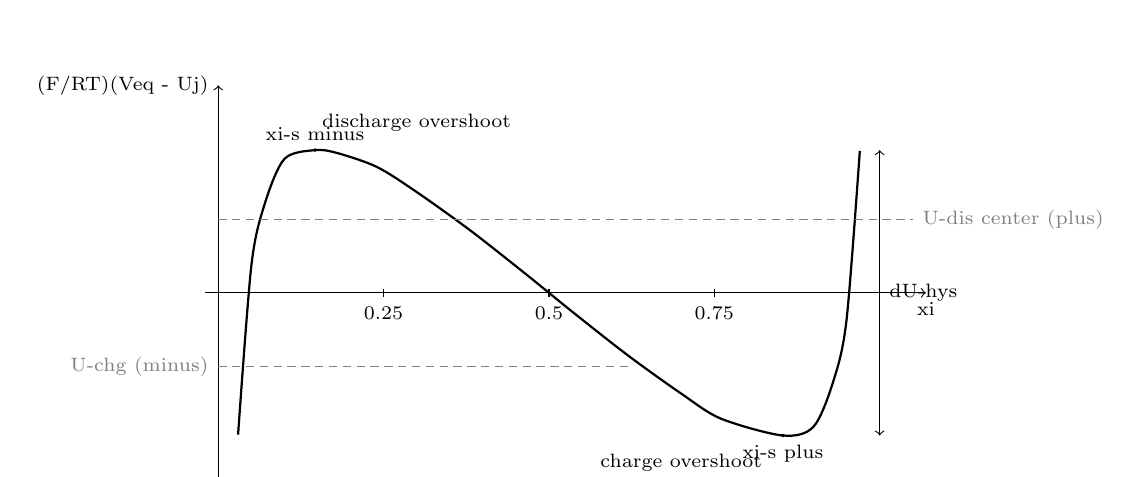
\begin{tikzpicture}[x=8.4cm,y=1.7cm]
% Non-monotone equilibrium potential V_eq(xi)-U_j (scaled by F/RT) for Omega=4RT.
% van der Waals-like loop; spinodal extrema mark branch supremum/infimum.
\draw[->] (0,-1.45) -- (0,1.55) node[left,font=\scriptsize] {(F/RT)(Veq - Uj)};
\draw[->] (-0.02,0) -- (1.07,0) node[below,font=\scriptsize] {xi};
\foreach \xx in {0.25,0.5,0.75} {\draw (\xx,0.03) -- (\xx,-0.03) node[below,font=\scriptsize] {\xx};}
\draw[thick] plot[smooth] coordinates {
 (0.03,-1.06)(0.05,0.20)(0.07,0.66)(0.10,1.00)(0.1464,1.066)
 (0.18,1.044)(0.24,0.94)(0.30,0.753)(0.38,0.470)(0.46,0.160)
 (0.50,0)(0.54,-0.160)(0.62,-0.470)(0.70,-0.753)(0.76,-0.94)
 (0.8536,-1.066)(0.90,-1.00)(0.93,-0.66)(0.95,-0.20)(0.97,1.06)};
% discharge overshoot path (left, up to spinodal max), branch center marker
\fill (0.1464,1.066) circle (0.7pt) node[above,font=\scriptsize] {xi-s minus};
\fill (0.8536,-1.066) circle (0.7pt) node[below,font=\scriptsize] {xi-s plus};
\draw[<->] (1.0,-1.066) -- (1.0,1.066) node[pos=0.5,right,font=\scriptsize] {dU-hys};
\draw[densely dashed,gray] (0.0,0.55) -- (1.05,0.55) node[right,font=\scriptsize] {U-dis center (plus)};
\draw[densely dashed,gray] (0.0,-0.55) -- (0.62,-0.55);
\node[left,font=\scriptsize,gray] at (0.0,-0.55) {U-chg (minus)};
\node[font=\scriptsize] at (0.30,1.27) {discharge overshoot};
\node[font=\scriptsize] at (0.70,-1.27) {charge overshoot};
\end{tikzpicture}
\caption{비단조 평형 전위 loop($\Omega_j=4RT$, 신규 작성)와 방향별 분기 중심. 곡선의 극값이 spinodal $\xi_s^\pm$(식~\eqref{eq:spinodal}); 두 극값의 차가 상한 gap $\Delta U^\hys$(식~\eqref{eq:dUhys}). 방전은 좌상으로 과주행, 충전은 우하로 거울 과주행해 중심이 $U_j\pm\tfrac12\gamma_j\Delta U^\hys$ 로 갈린다(식~\eqref{eq:Ubranch}; 회색 점선). $\gamma\to0$ 또는 $\Omega\le2RT$ 면 두 중심이 $U_j$ 로 합쳐진다.}
\label{fig:hysbranch}
\end{figure}

\begin{codebox}
\texttt{func\_dU\_hys(T,Omega)} [L123] — \texttt{Omega<=2RT} 면 \texttt{0.0}, 아니면 \texttt{(2/F)(Omega*u - 2RT*arctanh(u))}, \texttt{u=sqrt(1-2RT/Omega)}. \texttt{func\_U\_branch(T,U\_j,Omega,gamma,sigma\_d,h\_eta)=U\_j+0.5*sigma\_d*h\_eta*gamma*dU\_hys} [L133]. \texttt{dqdv} 는 \texttt{hys\_shift=func\_U\_branch(T\_rep,0.0,Omega,gamma,sigma\_d,h\_eta)}(전이당 상수)를 배열 \texttt{U\_j} 에 가산해 \texttt{center} 생성 [L448-454]; \texttt{gamma==0 or Omega<=0} 이면 \texttt{center=U\_j}. 부호 체크 4: $\Delta U^\hys\ge0$, $\Omega\le2RT\to0$, 분기 $\pm\tfrac12\sgn$ ✓.
\end{codebox}

% ====================================================================
\section{폭과 평형 점유 — logistic 등온선 (N4, N5)}\label{sec:width}
% ====================================================================
분기 중심 $U_j^d$ 가 정해졌으니, 코드는 폭 $w$ 를 정하고 평형 점유 $\xi_\eq$ 를 logistic 으로 친다. 이 두 양이 평형 종(N6)의 너비와 모양을 결정한다. logistic 형 자체는 속도식의 정지점에서 유도되므로 그 사슬을 둔다.

\subsection{폭 $w$ — 이상 극한과 $\Omega$-좁힘}
폭은 전이의 전위 스케일이다. 이상 극한($\Omega=0$)에서 폭은 열전압 $RT/F$ 에 다중도 $n$ 을 곱한 값:
\begin{equation}
w_j\;=\;n_j\,\frac{RT}{F}.
\label{eq:w}
\end{equation}
다중도는 코드가 \texttt{n} 직접 또는 \texttt{w} 에서 $n=wF/(RT)$ 역산으로 얻는다. 상호작용이 있으면 종이 좁아지는데, 평형 등온선 중심 기울기를 이상 logistic 과 같다고 두면(식~\eqref{eq:logistic} 의 중심 기울기 $\propto1/w$) 유효 폭이 나온다:
\begin{equation}
w_j^\eff\;=\;\frac{RT}{F}\Big(1-\frac{\Omega_j}{2RT}\Big),
\label{eq:weff}
\end{equation}
$\Omega_j\to2RT$ 에서 $0$(좁힘 임계), $\Omega_j=0$ 에서 $RT/F$ 회복. 일반 폭 $w_j$ 는 이 둘을 포괄하는 양이고, 코드는 기본적으로 $w_j=nRT/F$(식~\eqref{eq:w})를 쓴다. \texttt{use\_w\_eff} 를 켜고 그리고 \texttt{Omega} 가 있고 \texttt{w} 직접 지정이 없을 때만 식~\eqref{eq:weff} 로 좁히되, $RT/F$ 의 하한 분율 \texttt{floor\_frac}$=0.05$ 로 클립한다(폭 $0\to$ 발산 방지). 세 조건 가운데 마지막 ``\texttt{w} 직접 지정이 없을 것''이 실전에서 자주 걸린다 — 게이트 \texttt{\_width} 가 \texttt{tr.get('w') is None} 을 요구하므로, 전이 dict 에 \texttt{'w'} 키가 \emph{하나라도} 들어 있으면 \texttt{use\_w\_eff=True} 라도 $w^\eff$ 좁힘이 실효 없이 우회되고 폭은 그대로 $nRT/F$ 로 평가된다. 곧 \texttt{'w'} 키는 (다음에 볼 폭 다중도 $n$ 의 폴백일 뿐 아니라) $w^\eff$ 게이트의 차단키이기도 하다. $w^\eff$ 좁힘을 실제로 켜려면 전이 dict 에서 \texttt{'w'} 를 빼고 폭을 $\Omega$ 와 $n$ 으로만 주어야 한다(\S\ref{sec:sum} 의 \texttt{GRAPHITE\_STAGING\_LIT} 가 정확히 이 함정에 해당 — 네 전이가 모두 \texttt{'w'} 를 실어 좁힘이 무효다).

\subsection{logistic — 정$\cdot$역 속도 정지점에서 유도}
평형 점유율의 logistic 형은 가정이 아니라 속도식의 정지점이다. 구동력(affinity) $\mathcal A$ 는 전이가 평형에서 벗어난 자유에너지로, 식~\eqref{eq:gibbsdef} 의 $\Delta G_{\mathrm{rxn}}(V)=-F(V-U)$ 를 방향 부호로 부호 맞춘 $\mathcal A=\sgn F(V-U)$ 다($V=U$ 에서 $0$). 전이상태를 지나는 정$\cdot$역 속도는 이 $\mathcal A$ 가 두 장벽을 비대칭 이동시킨 것이라, 점유 인자(정방향은 찬 자리 $1-\xi$, 역방향은 빈 자리 $\xi$)를 붙인 운동방정식은
\begin{equation}
\frac{\dd\xi}{\dd t}=r^+(1-\xi)-r^-\xi=k(\xi_\eq-\xi),\qquad
\xi_\eq\equiv\frac{r^+}{r^++r^-},\quad \frac{r^+}{r^-}=e^{\mathcal A/RT}
\label{eq:relax}
\end{equation}
이다. 마지막 비는 detailed balance 다 — 고개의 분율 위치 $\chi$ 가 정$\cdot$역 장벽 비에서 약분되므로 $\chi$ 는 속도에만 들고 평형에는 들지 않는다. 정지점 $\xi_\eq/(1-\xi_\eq)=e^{\mathcal A/RT}$ 를 $\xi_\eq$ 로 풀고 $\mathcal A=\sgn F(V-U)$ 를 넣으면
\begin{equation}
\boxed{\;\xi_{\eq,j}(V,T)=\frac{1}{1+\exp\!\big[-\sgn(V-U_j^d)/w_j\big]}\;,\qquad
w_j=\frac{RT}{F}\ (\text{이상 극한})\;.}
\label{eq:logistic}
\end{equation}
부호 — 방전($\sgn=+1$)에서 $V>U_j^d\Rightarrow\xi_\eq\to1$(탈리튬화 완료 쪽), $V<U_j^d\Rightarrow0$, $V=U_j^d\Rightarrow\tfrac12$(전이 중심). 충전($\sgn=-1$)이면 logistic 인자 부호가 뒤집혀 진행 방향이 거울이다. 코드 \texttt{func\_ksi\_eq} 는 수치 안정형(양$\cdot$음 $z$ 분기)으로 같은 식을 평가하고, 격자 $V_\work$ 와 분기 중심 \texttt{center}$=U_j^d$ 를 받는다. 이 $\xi_\eq$ 가 다음 절 평형 peak 의 원천이다.

\begin{verifybox}
\textbf{극한$\cdot$수치.} $V\gg U\Rightarrow\xi_\eq\to1$, $V\ll U\Rightarrow0$, $V=U\Rightarrow\tfrac12$. $w=RT/F=25.7$ mV($25^\circ$C), $22.2$ mV($-15^\circ$C). $\Omega\to2RT$ 에서 $w^\eff\to0$(좁힘 임계, 식~\eqref{eq:weff}). 부호 체크 2: $\xi_\eq=\mathrm{logistic}[\sgn(V-U)/w]$, 방전 $V\!\uparrow\Rightarrow\xi\!\uparrow$ ✓.
\end{verifybox}

\begin{codebox}
\texttt{func\_w(T,n)=n*R*T/F} [L64], \texttt{func\_w\_eff(T,Omega,floor\_frac)} [L141] = \texttt{max((RT/F)(1-Omega/2RT), floor\_frac*RT/F)}. \texttt{\_width} [L283-288]: \texttt{use\_weff and tr.get('Omega') is not None and tr.get('w') is None} 일 때만 \texttt{func\_w\_eff}, 아니면 \texttt{func\_w}. ★\texttt{tr.get('w') is None} 게이트 — dict 에 \texttt{'w'} 키 있으면 \texttt{use\_w\_eff=True} 라도 $w^\eff$ 우회. \texttt{func\_ksi\_eq(T,V\_n,U,n,s)} [L84]: \texttt{z=s*(V\_n-U)/func\_w(T,n)}, \texttt{where(z>=0, 1/(1+exp(-z)), exp(z)/(1+exp(z)))}. \texttt{dqdv} 호출 L459: \texttt{ksi\_eq=func\_ksi\_eq(T\_work,V\_work,center,n\_j,sigma\_d)}.
\end{codebox}

% ====================================================================
\section{평형 peak — logistic 의 미분 ($|I|\to0$ 한계) (N6)}\label{sec:eqpeak}
% ====================================================================
평형 점유 $\xi_\eq$ 에서 평형 $\dd Q/\dd V$ 가 바로 나온다 — 코드가 저율$\cdot|I|\to0$ 에서 직접 쓰는 종 모양이고, 동시에 \texttt{equilibrium} 기준선 메서드의 본체다. 이 기준선이 있어야 전류가 흐를 때의 변화를 이탈(N7$\cdot$N8)로 읽는다.

\subsection{종 모양 — $\xi(1-\xi)/w$}
관측 $\dd Q/\dd V$ 는 전하 보존식 $Q_\cell q=Q_\bg(V_n)+\sum_jQ_j\xi_j$ 를 궤적으로 미분한 $C_\bg+\sum_jQ_j\,\dd\xi_j/\dd V_n$ 이다. 평형 추종이면 $\xi_j=\xi_{\eq,j}$ 이므로 logistic 의 미분이 들어간다. $z\equiv\sgn(V-U_j^d)/w_j$ 로 두고 $\xi_\eq=(1+e^{-z})^{-1}$ 를 미분하면 항등식
\begin{equation}
\frac{\dd\xi_\eq}{\dd z}=\frac{e^{-z}}{(1+e^{-z})^2}=\xi_\eq(1-\xi_\eq)
\label{eq:belliden}
\end{equation}
이 나오고, 연쇄율 $\dd z/\dd V=\sgn/w_j$ 를 곱하면
\begin{equation}
\frac{\dd\xi_{\eq,j}}{\dd V}=\frac{\sgn\,\xi_{\eq,j}(1-\xi_{\eq,j})}{w_j}.
\label{eq:dxidV}
\end{equation}
부호 — 식~\eqref{eq:dxidV} 에서 $\xi(1-\xi)>0$ 이고 $1/w_j>0$ 이라, $\sgn$ 이 곱해져도 $Q_j\,\dd\xi_j/\dd V$ 에 들어가는 peak 기여는 \textbf{양수}다(방전$\cdot$충전 방향 불변; 충전은 진행축이 거울이라 같은 양수 peak 를 남긴다). 그래서 코드의 평형 peak 항은 $\sgn$ 없이 $\xi_\eq(1-\xi_\eq)/w$ 로 적힌다:
\begin{equation}
\boxed{\;\Big(\frac{\dd Q}{\dd V}\Big)^{\eq}_j=Q_j\,\frac{\xi_{\eq,j}(1-\xi_{\eq,j})}{w_j}
=Q_j\,\Big|\frac{\dd\xi_{\eq,j}}{\dd V}\Big|\;.}
\label{eq:eqpeak}
\end{equation}
$\xi(1-\xi)$ 는 $\xi=\tfrac12$ 에서 최대 $\tfrac14$ 인 종이라, peak 위치 $=U_j^d$, 순높이 $=Q_j/(4w_j)$, 배경 차감 면적 $=Q_j$($\int_0^1\dd\xi=1$)다. 저온일수록 $w\propto T$ 라 평형 peak 는 좁고 높다(면적 보존) — 관측이 정반대(저온에서 넓고 낮음)면 그 역전이 동역학 꼬리(N7$\cdot$N8)의 증거다.

\subsection{기준선 메서드 — $|I|\to0$ 한계}
$|I|\to0$ 이면 꼬리 길이 $L_V\to0$(N7)이라 지연이 사라지고 식~\eqref{eq:eqpeak} 만 남는다. 코드의 \texttt{equilibrium} 메서드가 이 합이다:
\begin{equation}
\Big(\frac{\dd Q}{\dd V}\Big)^\eq=C_\bg+\sum_{j=1}^{N_p}Q_j\,\frac{\xi_{\eq,j}(1-\xi_{\eq,j})}{w_j}
\qquad(|I|\to0,\ \text{충방전 불변}\cdot\text{히스 미반영}).
\label{eq:equilibrium}
\end{equation}
이것이 동역학을 켜기 전의 기준선이다. 단 \texttt{equilibrium} 은 분기 미반영($U_j$ 중심)이라, $\gamma>0$ 전이에서는 \texttt{dqdv} 의 $|I|\to0$ 극한(분기 중심 $U_j^d$, 식~\eqref{eq:Ubranch})과 중심이 $\pm\tfrac12\gamma\Delta U^\hys$ 만큼 다르다 — 두 메서드가 완전히 일치하는 것은 $\gamma=0$ 또는 $\Omega\le2RT$ 일 때다. 그림~\ref{fig:bell} 가 logistic 과 그 미분 종을 겹쳐 보인다.

\begin{figure}[t]
\centering
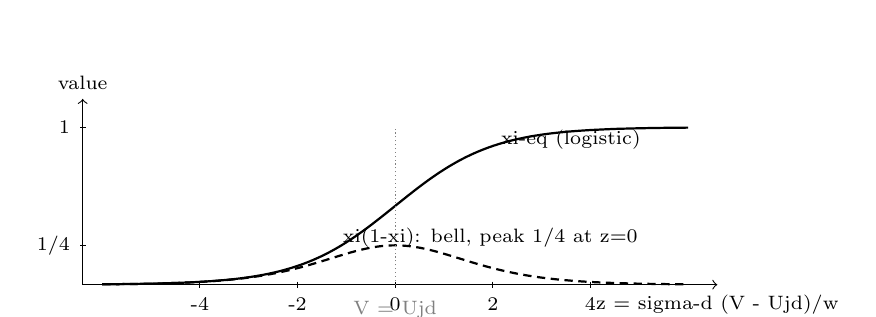
\begin{tikzpicture}[x=0.62cm,y=2.0cm]
% logistic xi_eq(z) and its derivative bell xi(1-xi) on z=(V-Ud)/w axis
\draw[->] (-6.4,0) -- (6.6,0) node[below,font=\scriptsize] {z = sigma-d (V - Ujd)/w};
\draw[->] (-6.4,0) -- (-6.4,1.18) node[above,font=\scriptsize] {value};
\foreach \zz in {-4,-2,0,2,4} {\draw (\zz,0.02) -- (\zz,-0.02) node[below,font=\scriptsize] {\zz};}
\draw (-6.34,1.0) -- (-6.46,1.0) node[left,font=\scriptsize] {1};
\draw (-6.34,0.25) -- (-6.46,0.25) node[left,font=\scriptsize] {1/4};
% logistic curve
\draw[thick] plot[smooth,samples=60,domain=-6:6] (\x,{1/(1+exp(-\x))});
% derivative bell xi(1-xi)
\draw[thick,densely dashed] plot[smooth,samples=60,domain=-6:6] (\x,{exp(-\x)/(1+exp(-\x))/(1+exp(-\x))});
\node[font=\scriptsize] at (3.6,0.92) {xi-eq (logistic)};
\node[font=\scriptsize] at (1.95,0.30) {xi(1-xi): bell, peak 1/4 at z=0};
\draw[densely dotted,gray] (0,0) -- (0,1.0);
\node[below,font=\scriptsize,gray] at (0,-0.04) {V = Ujd};
\end{tikzpicture}
\caption{평형 점유 logistic(실선, 식~\eqref{eq:logistic})과 그 미분 종 $\xi(1-\xi)$(파선, 식~\eqref{eq:belliden}; 신규 작성). 종은 중심 $V=U_j^d$($z=0$)에서 최대 $\tfrac14$, 폭 척도 $w$. 평형 peak(식~\eqref{eq:eqpeak})은 이 종에 $Q_j/w$ 를 곱한 것이라 순높이 $Q_j/(4w)$$\cdot$면적 $Q_j$. $\sgn$ 은 $z$ 안에서 진행축만 거울로 바꾸고 종 자체(따라서 peak 부호)는 방향 불변이다.}
\label{fig:bell}
\end{figure}

\begin{codebox}
\texttt{equilibrium(V\_n,T)} [L354]: \texttt{dqdv = baseline}, \texttt{for tr: dqdv += tr['Q']*ksi\_eq*(1-ksi\_eq)/w} [L370]. \texttt{dqdv} 의 저지연 분기 [L468]: \texttt{peak\_shape = ksi\_eq*(1-ksi\_eq)/w} ($\sgn$ 없음 — 방향 불변). 부호 체크 3: $\dd\xi/\dd V=\sgn\,\xi(1-\xi)/w$, peak 양수 ✓.
\end{codebox}

% ====================================================================
\section{동역학 지연 길이 — 컷 affinity·유효 장벽·$L_V$ (N7)}\label{sec:lag}
% ====================================================================
평형 peak 기준선 다음에 코드는 전류가 만드는 지연 길이 $L_V$ 를 전이당 한 번 산출한다 — 컷 affinity $\mathcal A$, 방향별 전달계수 $\chi_d$, 유효 장벽 $\Delta H_a^\eff$ 를 거쳐 $L_q$ 를 얻고 전압축으로 환산한다. C-rate 세 인자가 전부 이 한 양을 통해 꼬리로 들어온다.

\subsection{지연의 보편 방정식과 길이 $L_q$}
정전류에서 $\dd q/\dd t=|I|/Q_\cell$ 이고, 운동방정식~\eqref{eq:relax} 을 이로 나누면 지연 $r_j\equiv\xi_{\eq,j}-\xi_j$ 의 보편 방정식이 나온다:
\begin{equation}
\frac{\dd r_j}{\dd q}=\frac{\dd\xi_{\eq,j}}{\dd q}-\frac{r_j}{L_{q,j}},\qquad
L_{q,j}=\frac{|I|}{Q_\cell\,k_j}.
\label{eq:Lq}
\end{equation}
첫 항은 평형 목표 이동의 지연 공급, 둘째는 완화의 소거다. 길이 $L_{q,j}$ 는 요구($|I|/Q_\cell$)/공급($k_j$) 비 그 자체다. 완화 속도의 보편형은 정$\cdot$역 합 $k_j=r_j^++r_j^-=r_j^+(1+e^{-\mathcal A_j/RT})$ 이고($r_j^-=r_j^+e^{-\mathcal A_j/RT}$, detailed balance), 정방향은 식~\eqref{eq:relax} 의 비대칭 장벽에서 $r_j^+=k_0e^{-(\Delta G_a-\chi_d\mathcal A)/RT}$($k_0=k_BT/h$, 방향별 $\chi_d$)이다. 이 보편 $k_j$ 를 $L_{q,j}=|I|/(Q_\cell k_j)$ 에 넣으면 닫힌 꼴이 나온다:
\begin{equation}
L_{q,j}\;=\;\frac{|I|}{Q_\cell}\cdot\frac{h}{k_BT}\,
\exp\!\Big[\frac{\Delta G_{a,j}^\eff-\chi_d\mathcal A_j}{RT}\Big]\cdot\frac{1}{1+e^{-\mathcal A_j/RT}},
\qquad \Delta G_{a,j}^\eff=\Delta H_{a,j}^\eff-T\Delta S_{a,j}.
\label{eq:Lqclosed}
\end{equation}
마지막 인자 $1/(1+e^{-\mathcal A/RT})$ 는 보편 $k_j$ 의 역방향 몫(괄호)이 분모로 들어간 전이대 보정이고, 꼬리($\mathcal A\gtrsim3RT$)에서 1로 죽어 forward 극한 $k_j\simeq r_j^+$ 가 회복된다. 유효 장벽 $\Delta H_a^\eff$ 는 아래에서 닫는다. 전위 의존 — $\partial\ln L_q/\partial V=-\chi_d\sgn F/RT\le0$($\sgn=+1$), 곧 \textbf{전위$\uparrow\Rightarrow$장벽$\downarrow\Rightarrow$꼬리$\downarrow$}(부호 체크 6).

\subsection{컷 affinity $\mathcal A$ — 정점의 5\% 컷}
꼬리는 한 점에서 평가한다 — 식~\eqref{eq:relax} 의 affinity $\mathcal A=\sgn F(V-U)$ 를, 평형 종 미분 $\xi_\eq(1-\xi_\eq)$ 가 정점의 일정 분율($5\%$)로 떨어지는 컷점에서 평가한 크기다. 그 컷의 logit 위치는 $\xi(1-\xi)=0.0125$ 의 큰 근에서 $z\equiv|V-U|/w\approx4.357$ 이고, $w=nRT/F$ 라 $|\mathcal A|/RT=|F(V-U)|/RT=n\,z\approx z_{\mathrm{cut}}\,n$($z_{\mathrm{cut}}=4.357$). affinity 크기는 \emph{충$\cdot$방전 동일}로 두고 방향은 아래 $\chi_d\cdot\Delta H_a^\eff$ 가 받는다(부호는 컷 밖). 폭 다중도 $n$ 과 affinity$\cdot$꼬리 길이는 전이당 한 번 대표 온도 $T_\rep$$\cdot$$|n|$ 에서 평가한다(격자 점별 대입 X):
\begin{equation}
\mathcal A=\min\big(z_{\mathrm{cut}}\,|n|\,RT,\ A_{\mathrm{cap}}\,RT\big),\qquad z_{\mathrm{cut}}=4.357,\ \ A_{\mathrm{cap}}=4.
\label{eq:affcut}
\end{equation}
상한 $A_{\mathrm{cap}}\,RT$ 가 폭이 큰 전이에서 컷이 과도하게 깊어지는 것을 막는다. $\mathcal A$ 를 $\min$ 안에 양수 크기로 둔 것이 핵심이다 — $\sgn$ 을 $\min$ 안에 두면 충전에서 음수 상한이 돼 버리는 부호 버그를 피한 형태다.

\subsection{방향별 전달계수와 유효 장벽}
전달계수 $\chi$ 는 고개의 분율 위치이고, 정$\cdot$역 합이 1로 강제된다(detailed balance). 꼬리가 깊은 쪽이 방전($\xi\to1$)과 충전($\xi\to0$)에서 거울이라 역방향 장벽의 상수 몫이 갈리므로, 방향별 전달계수는
\begin{equation}
\chi_d=\mathrm{chi\_split}(\chi,\sgn)=\begin{cases}\chi & \sgn\ge0\ (\text{방전})\\ 1-\chi & \sgn<0\ (\text{충전})\end{cases}
\label{eq:chid}
\end{equation}
다(코드는 이 규칙을 주입 가능한 callable 로 노출, 기본 \texttt{func\_chi\_d}). 깊은 꼬리에서 상호작용 상수 몫 $+\Omega$ 가 장벽에 흡수돼 유효 활성화 엔탈피가 된다:
\begin{equation}
\boxed{\;\Delta H_{a,j}^\eff=\Delta H_{a,j}-\chi_d\,\Omega_j\;.}
\label{eq:dHeff}
\end{equation}
방향별($\chi_d$)이라 충$\cdot$방전 꼬리 길이가 갈린다(부호 체크 5). \texttt{use\_dH\_eff} 가 꺼지면 $\Delta H_a^\eff=\Delta H_a$.

\subsection{$L_q\to L_V$ 환산}
$L_q$ 는 코드 함수 \texttt{func\_L\_q} 가 식~\eqref{eq:Lqclosed} 의 로그형으로 평가하고(인자 \texttt{x} 자리에 $\chi_d$, \texttt{A} 자리에 컷 $\mathcal A$, 장벽 자리에 $\Delta H_a^\eff$), 전압축 길이는 컷점 OCV 기울기로 환산한다:
\begin{equation}
\boxed{\;L_{V,j}=\Big|\frac{\dd V}{\dd q}\Big|_{q_a}\,L_{q,j}\;.}
\label{eq:LV}
\end{equation}
기울기 $|\dd V/\dd q|_{q_a}$ 는 코드 전이 dict 의 \texttt{dVdq\_qa}(컷 OCV 기울기, 피팅값)다. $|I|\to0^+$ 이면 $L_q\propto|I|\to0$ 이라 $L_V\to0$, 다음 절 인과 꼬리가 평형 peak 로 환원된다. 코드는 $|I|\le0$ 또는 동역학 키(\texttt{dH\_a}) 부재 시 $L_V$ 를 $0$ 으로 단락하고(평형 종 직접), 함수 \texttt{func\_L\_q} 자체는 $I\le0$ 에서 $-\infty$(미정의)를 반환하므로 재현 코드는 이 컷을 둬야 한다. 전이 dict 에 \texttt{L\_V} 직접 지정이 있으면 동역학을 우회한다(피팅$\cdot$테스트용). 이 $L_V$ 가 다음 절의 인과 저역통과 커널 길이로 넘어가, 평형 점유를 지연시켜 꼬리를 만든다.

\begin{verifybox}
\textbf{컷$\cdot$차원.} $\xi(1-\xi)$ 가 정점($\xi=\tfrac12$)의 $5\%$ 로 떨어지는 $z$ — $\xi(1-\xi)=0.0125$ 의 큰 근에서 $z\approx4.36$, 코드 $z_{\mathrm{cut}}=4.357$ 정합. $L_q$ 무차원 — $(|I|/Q_\cell)$ [1/s] $\times$ $h/(k_BT)$ [s] $=$ 무차원 ✓. 부호 체크 6: $\partial\ln L_q/\partial V=-\chi_d\sgn F/RT<0$($\sgn=+1$) ✓ — 이는 affinity 의 \emph{연속} 전위 의존(꼬리가 깊을수록 짧아짐)이고, 코드는 이를 전이당 한 점(컷)에서 동결해 쓴다.
\end{verifybox}

\begin{codebox}
\texttt{\_resolve\_lag\_length} [L307]: \texttt{L\_V} 직접이면 반환; \texttt{I<=0 or dH\_a None} 이면 \texttt{0.0}. \texttt{A=min(z\_cut*n\_safe*R*T, A\_cap*R*T)} [L335]. \texttt{chi\_d,dH\_a\_use=\_chi\_and\_dH\_eff(...)} (= \texttt{func\_dH\_a\_eff} 또는 raw). \texttt{L\_q=func\_L\_q(T,I,Q\_cell,dH\_a\_use,dS\_a,chi\_d,A)} [L346], \texttt{func\_L\_q} [L90]: \texttt{ln\_Lq=ln(T\_attempt/T)-ln(1+exp(-A/RT))+dG\_a/RT - x*A/RT}, \texttt{T\_attempt=(I/Q\_cell)*h/kB}. 반환 \texttt{abs(dVdq\_qa)*L\_q} [L351]. \texttt{func\_chi\_d} [L155], \texttt{func\_dH\_a\_eff} [L149]. 부호 체크 5: $\chi_d$(방전 $\chi$/충전 $1-\chi$), $\Delta H_a^\eff=\Delta H_a-\chi_d\Omega$ ✓.
\end{codebox}

% ====================================================================
\section{인과 기억 꼬리 — 지수 저역통과와 충전 격자 역전 (N8)}\label{sec:tail}
% ====================================================================
지연 길이 $L_V$ 가 정해지면, 코드는 평형 점유 $\xi_\eq$ 를 인과 지수 커널로 저역통과시켜 지연 점유 $\xi_\lagg$ 를 만들고, 그 차로 peak 모양을 짓는다. 이 절의 핵심은 \textbf{충전의 격자 역전}이다 — 진행 방향이 반대인 충전에서 인과성을 보존하는 장치.

\subsection{지수 기억 — 보편 방정식의 일반해}
지연 방정식~\eqref{eq:Lq} 은 1계 선형이라 적분인자 $e^{q/L_q}$ 로 닫힌 해를 갖고, 초기 지연이 사멸한 뒤의 해는 과거 목표 변화율을 지수 커널로 가중한 합성곱이다:
\begin{equation}
r_j(q)=\int_{-\infty}^{q}e^{-(q-q')/L_{q,j}}\,\frac{\dd\xi_{\eq,j}}{\dd q'}\,\dd q',
\qquad K(\Delta q)=e^{-\Delta q/L_{q,j}}\ (\Delta q\ge0).
\label{eq:memory}
\end{equation}
계는 용량축에서 길이 $L_q$ 만큼의 최근 과거만 기억한다. 용량축 커널을 전압축으로 옮기면 $\Delta q=\Delta V/|\dd V/\dd q|$ 와 $L_q\to L_V=|\dd V/\dd q|L_q$ 가 짝이라 $\Delta q/L_q=\Delta V/L_V$ — 곧 감쇠율이 전압축에서도 $a=e^{-\Delta V/L_V}$ 로 불변이다. 이산화하면 격자 간격 $\Delta V$$\cdot$전압축 길이 $L_V$ 의 1극 IIR 저역통과가 되고, 지연 점유 $\xi_\lagg$ 는
\begin{equation}
\xi_\lagg[i]=a\,\xi_\lagg[i-1]+(1-a)\,\xi_\eq[i],\qquad a=e^{-\Delta V/L_V}.
\label{eq:lowpass}
\end{equation}
코드 \texttt{\_causal\_lowpass} 가 이 점화식(또는 등가 \texttt{scipy.signal.lfilter})을 평가한다. ``인과''는 현재 출력이 과거 입력에만 의존한다는 뜻 — 필터가 격자를 \emph{오름차순}으로 훑는다.

\subsection{★충전 격자 역전 — 진행 방향의 과거를 기억}
인과 합성곱~\eqref{eq:memory} 은 ``진행 방향의 과거''를 기억한다. 방전($\sgn=+1$)은 진행이 $V$ 증가라 격자 오름차순이 곧 시간순이므로 점화식~\eqref{eq:lowpass} 를 그대로 적용한다. 충전($\sgn=-1$)은 진행이 $V$ \emph{감소}라 시간순이 격자 \emph{내림차순}이다 — 오름차순 필터를 그대로 쓰면 미래를 기억하는 비인과가 된다. 그래서 충전은 격자를 뒤집어 필터한 뒤 되돌린다:
\begin{equation}
\boxed{\;\xi_\lagg=\begin{cases}
\mathrm{lowpass}(\xi_\eq,\,\Delta V,\,L_V) & \sgn\ge0\ (\text{방전})\\[2pt]
\mathrm{lowpass}\big(\xi_\eq[::\!-\!1],\,\Delta V,\,L_V\big)[::\!-\!1] & \sgn<0\ (\text{충전})
\end{cases}\;}
\label{eq:reversal}
\end{equation}
이 역전이 충전 $\dd Q/\dd V$ 를 방전의 \emph{거울}로 만든다 — 꼬리가 충전 진행 방향(저전위 쪽)으로 끌리되 부호는 양수를 유지한다(부호 체크 7).

\subsection{peak 모양 — 평형에서 지연을 뺀 것}
지연 점유가 정해지면 peak 모양은 평형과 지연의 차를 $L_V$ 로 나눈 이산 미분이다:
\begin{equation}
\boxed{\;\text{peak\_shape}=\frac{\xi_{\eq,j}-\xi_{\lagg,j}}{L_{V,j}}\;.}
\label{eq:peakshape}
\end{equation}
이것이 식~\eqref{eq:eqpeak} 의 평형 종을 일반화한 ``평형 전환율에서 지연을 뺀 것의 미분''이다. $L_V$ 가 작으면($L_V<m\,\Delta V$, $m=$ 최소 지연 격자수 \texttt{min\_lag\_grid\_steps}$=2.0$) 저역통과가 거의 항등이라 $\xi_\eq-\xi_\lagg\to L_V\,\dd\xi_\eq/\dd V$ 가 돼 식~\eqref{eq:peakshape} 가 평형 종 $\xi_\eq(1-\xi_\eq)/w$ 로 환원된다 — 코드가 저지연 분기에서 평형 종을 직접 쓰는 근거다. $L_V$ 가 크면 상승부가 기억에 덮여 정점이 늦고 낮아지며 긴 꼬리를 남긴다. 그림~\ref{fig:tail} 가 방전$\cdot$충전 꼬리의 거울 방향을 보인다.

\begin{figure}[t]
\centering
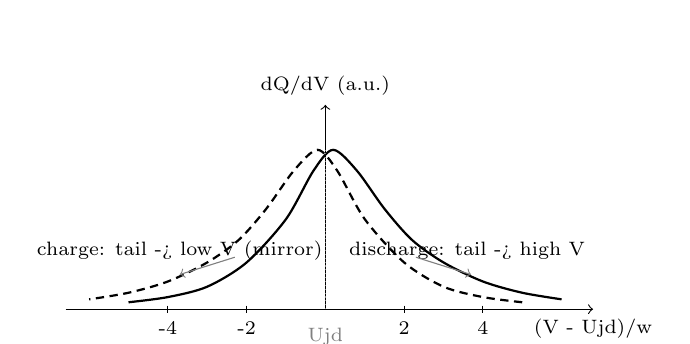
\begin{tikzpicture}[x=0.50cm,y=2.2cm]
% discharge: equilibrium bell + tail to the right (high V). charge: mirror, tail to left.
\draw[->] (-6.6,0) -- (6.8,0) node[below,font=\scriptsize] {(V - Ujd)/w};
\draw[->] (0,0) -- (0,1.18) node[above,font=\scriptsize] {dQ/dV (a.u.)};
\foreach \zz in {-4,-2,2,4} {\draw (\zz,0.02) -- (\zz,-0.02) node[below,font=\scriptsize] {\zz};}
% discharge tail (right): bell skewed with exponential tail toward +
\draw[thick] plot[smooth] coordinates {
 (-5,0.04)(-4,0.07)(-3,0.13)(-2,0.27)(-1,0.52)(-0.3,0.80)(0.2,0.92)
 (0.8,0.80)(1.5,0.58)(2.2,0.40)(3,0.27)(4,0.16)(5,0.095)(6,0.057)};
\node[font=\scriptsize] at (3.6,0.34) {discharge: tail -> high V};
\draw[->,gray] (2.3,0.30) -- (3.7,0.20);
% charge tail (left): mirror
\draw[thick,densely dashed] plot[smooth] coordinates {
 (5,0.04)(4,0.07)(3,0.13)(2,0.27)(1,0.52)(0.3,0.80)(-0.2,0.92)
 (-0.8,0.80)(-1.5,0.58)(-2.2,0.40)(-3,0.27)(-4,0.16)(-5,0.095)(-6,0.057)};
\node[font=\scriptsize] at (-3.7,0.34) {charge: tail -> low V (mirror)};
\draw[->,gray] (-2.3,0.30) -- (-3.7,0.20);
\draw[densely dotted,gray] (0,0) -- (0,0.92);
\node[below,font=\scriptsize,gray] at (0,-0.05) {Ujd};
\end{tikzpicture}
\caption{인과 기억 꼬리의 방향(신규 작성). 실선 $=$ 방전($\sgn=+1$): 진행이 $V$ 증가라 꼬리가 고전위 쪽으로 끌린다. 파선 $=$ 충전($\sgn=-1$): 격자 역전(식~\eqref{eq:reversal})으로 거울 — 꼬리가 저전위 쪽으로 끌리되 부호는 양수 유지. 두 곡선 모두 $L_V$ 가 작으면 중심 $U_j^d$ 의 대칭 종(평형 peak, 식~\eqref{eq:eqpeak})으로 환원된다. peak 모양은 평형에서 지연을 뺀 것의 미분(식~\eqref{eq:peakshape}).}
\label{fig:tail}
\end{figure}

\begin{codebox}
\texttt{\_causal\_lowpass(source,grid\_step,lag\_length)} [L100]: \texttt{decay=exp(-grid\_step/lag\_length)}, \texttt{lfilter([1-decay],[1,-decay],...)} (fallback 점화식 L114-118). \texttt{dqdv} 분기 [L466-479]: \texttt{lag\_len\_V < min\_lag\_grid\_steps*grid\_step} 이면 평형 종; 아니면 \texttt{sigma\_d>=0: occ\_lagged=\_causal\_lowpass(ksi\_arr,...)}, else \texttt{\_causal\_lowpass(ksi\_arr[::-1],...)[::-1]} [L474-477], \texttt{peak\_shape=(ksi\_eq-occ\_lagged)/lag\_len\_V} [L479]. 부호 체크 7: 충전 격자 역전 $\xi[::\!-\!1]\cdots[::\!-\!1]$, 충전 $\dd Q/\dd V$ 방전 거울$\cdot$양수 ✓.
\end{codebox}

% ====================================================================
\section{합산과 역보간 — 네 전이의 ICA (N9)}\label{sec:sum}
% ====================================================================
전이 루프가 각 전이의 peak 모양을 만들면, 코드는 이를 용량 가중해 더하고 마지막에 측정축 $V_n$ 으로 역보간한다. 전하 보존식이 $\sum_jQ_j\xi_j$ 꼴이라 합산 자체는 보존의 직접 미분이다.

\subsection{합산식 — 평형 peak 에서 지연 꼬리를 뺀 것의 합}
작업 격자 위에서 배경에 전이별 기여를 누적하고, $V_n$ 으로 역보간한다:
\begin{equation}
\boxed{\;\frac{\dd Q}{\dd V}(V_n)=C_\bg+\sum_{j=1}^{N_p}Q_j\cdot\text{peak\_shape}_j
=C_\bg+\sum_{j=1}^{N_p}Q_j\,\frac{\xi_{\eq,j}-\xi_{\lagg,j}}{L_{V,j}}\;.}
\label{eq:total}
\end{equation}
저지연 전이는 $\text{peak\_shape}_j=\xi_{\eq,j}(1-\xi_{\eq,j})/w_j$(평형 종)로, 동역학 전이는 식~\eqref{eq:peakshape} 의 인과 꼬리로 들어간다. 각 항이 양수(평형 peak 의 방향 불변 양수성, 부호 체크 3)라 합도 양수다. 코드는 작업 격자 \texttt{dqdv\_work} 에 누적한 뒤 \texttt{np.interp(V\_n, V\_work, dqdv\_work)} 로 관측 격자에 되돌린다 — 작업 격자의 pad 여유(식~\eqref{eq:vwork})가 꼬리를 잘리지 않게 받은 뒤의 복귀다. 네 전이가 합쳐져 한 ICA 곡선이 되는 모습을 그림~\ref{fig:sum} 에 둔다.

\begin{figure}[t]
\centering
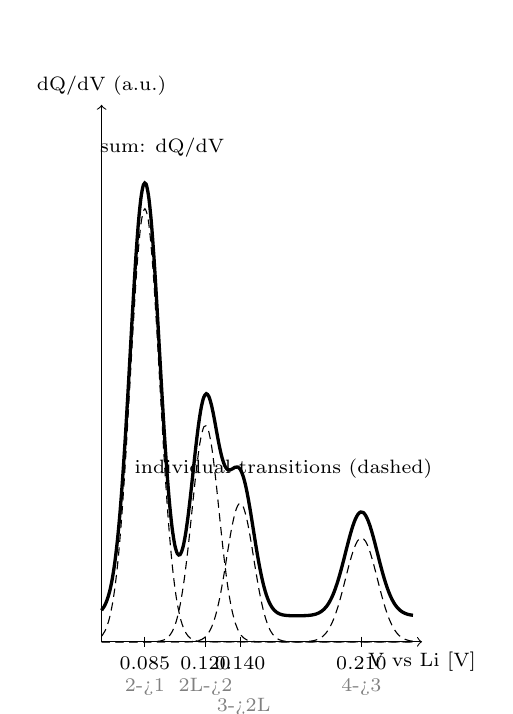
\begin{tikzpicture}[x=22.0cm,y=11.0cm]
% dQ/dV vs V (V from ~0.07 to 0.24). Four equilibrium-like bells at U=0.085,0.120,0.140,0.210
% with weights Q=0.50,0.25,0.12,0.10 and a common width; sum drawn as the heavy envelope.
% Use gaussian-like proxies for the bells (visual only; ASCII labels).
\def\bell#1#2#3{exp(-((\x-#1)/#2)^2)*#3}
\draw[->] (0.06,0) -- (0.245,0) node[below,font=\scriptsize] {V vs Li  [V]};
\draw[->] (0.06,0) -- (0.06,0.62) node[above,font=\scriptsize] {dQ/dV  (a.u.)};
\foreach \vv in {0.085,0.120,0.140,0.210} {\draw (\vv,0.006) -- (\vv,-0.006) node[below,font=\scriptsize] {\vv};}
% individual transition bells (thin)
\draw[densely dashed] plot[smooth,samples=80,domain=0.06:0.24] (\x,{\bell{0.085}{0.012}{0.50}});
\draw[densely dashed] plot[smooth,samples=80,domain=0.06:0.24] (\x,{\bell{0.120}{0.011}{0.25}});
\draw[densely dashed] plot[smooth,samples=80,domain=0.06:0.24] (\x,{\bell{0.140}{0.011}{0.16}});
\draw[densely dashed] plot[smooth,samples=80,domain=0.06:0.24] (\x,{\bell{0.210}{0.013}{0.12}});
% sum envelope (heavy)
\draw[very thick] plot[smooth,samples=120,domain=0.06:0.24]
  (\x,{\bell{0.085}{0.012}{0.50}+\bell{0.120}{0.011}{0.25}+\bell{0.140}{0.011}{0.16}+\bell{0.210}{0.013}{0.12}+0.03});
\node[font=\scriptsize] at (0.095,0.57) {sum: dQ/dV};
\node[font=\scriptsize] at (0.165,0.20) {individual transitions (dashed)};
\node[font=\scriptsize,gray] at (0.085,-0.052) {2->1};
\node[font=\scriptsize,gray] at (0.120,-0.052) {2L->2};
\node[font=\scriptsize,gray] at (0.142,-0.075) {3->2L};
\node[font=\scriptsize,gray] at (0.210,-0.052) {4->3};
\end{tikzpicture}
\caption{네 staging 전이의 합산(N9, 신규 작성; 형상은 도식). 파선 $=$ 전이별 기여 $Q_j\cdot$peak\_shape$_j$(중심 $U_j^d$, 면적 $\propto Q_j$), 굵은 실선 $=$ 합 $C_\bg+\sum_jQ_j\,$peak\_shape$_j$(식~\eqref{eq:total}; 배경 $C_\bg$ 만큼 들린다). 용량 가중 $Q$ 가 큰 $2\!\to\!1$ 전이가 가장 높고, 인접 전이($3\!\to\!2\mathrm L$, $2\mathrm L\!\to\!2$)는 중심이 가까워 부분 융합한다. 저온$\cdot$고율이면 각 꼬리(N8)가 길어져 골이 메워지고 분리 판독이 지워진다.}
\label{fig:sum}
\end{figure}

\subsection{staging 4전이 — \texttt{GRAPHITE\_STAGING\_LIT}}
흑연은 $N_p=4$ 전이다. 코드의 초기값 데이터셋 \texttt{GRAPHITE\_STAGING\_LIT} 가 네 전이의 인자를 담는다(피팅 override 전제의 시작점):
\begin{center}
\renewcommand{\arraystretch}{1.25}
\begin{tabular}{l c c c c c c}
\toprule
전이 & $U$ [V] & $Q$ [$Q_\cell$] & $\Delta H_{\mathrm{rxn}}$ & $\Delta S_{\mathrm{rxn}}$ & $\Delta H_a$ & $\Omega$ \\
 & ($U(298)$) & & [J/mol] & [J/mol/K] & [J/mol] & [J/mol] \\
\midrule
4$\to$3   & 0.210 & 0.10 & $-11700$ & $+29$ & $48000$ & $6000$ \\
3$\to$2L  & 0.140 & 0.12 & $-13500$ & $0$   & $46000$ & $8000$ \\
2L$\to$2  & 0.120 & 0.25 & $-13100$ & $-5$  & $44000$ & $10000$ \\
2$\to$1   & 0.085 & 0.50 & $-13000$ & $-16$ & $40000$ & $13000$ \\
\bottomrule
\end{tabular}
\end{center}
공통 인자 — $n=1$, $\Delta S_a=0$, \texttt{dVdq\_qa}$=0.30$ V(컷 OCV 기울기, fit). $\Delta H_{\mathrm{rxn}}/\Delta S_{\mathrm{rxn}}$ 은 각 전이의 $U(298)$ 목표(0.210/0.140/0.120/0.085 V)에 정합하도록 정한 열역학 값, $\Delta H_a$ 는 DFT 활성화(저SOC$\to$만충 감소 경향), $\Omega$ 는 정규용액 추정이다. 이 값들은 \emph{초기값}일 뿐 — 사용자 피팅이 override 한다(신뢰값 아님). 코드 dict 의 \texttt{'w'} 값($0.020$/$0.016$/$0.014$/$0.012$)은 \texttt{'n'} 이 있으면 쓰이지 않는 하위호환 폴백이다(\texttt{\_n\_factor} 가 \texttt{n} 우선) — 표는 유효값 $n=1$ 만 싣고, 폭은 $w=nRT/F$ 로 평가된다. 다만 이 \texttt{'w'} 키의 존재는 한 가지 부수효과를 갖는다 — \S\ref{sec:width} 에서 본 $w^\eff$ 게이트(\texttt{\_width} 의 \texttt{tr.get('w') is None} 조건)를 막는다. 곧 이 네 전이는 \texttt{'w'} 를 싣고 있어, \texttt{use\_w\_eff=True} 로 모델을 만들어도 $\Omega$-좁힘(식~\eqref{eq:weff})이 실효 없이 우회되고 폭은 그대로 $nRT/F$ 다. $w^\eff$ 좁힘을 실제로 적용해 피팅하려면 각 전이 dict 에서 \texttt{'w'} 를 빼고 $\Omega$$\cdot$$n$ 만으로 폭을 주어야 한다.

\subsection{이 문건만으로 곡선을 재현하려면 (G-usable)}
한 곡선은 다음 진행으로 닫힌다 — (1) 실험조건 $\to$ $\sgn,|I|,T,Q_\cell$(식~\eqref{eq:setup}); (2) $V_n=V_\app-\sgn|I|R_n$, 작업 격자 $V_\work$(pad)$\cdot\Delta V\cdot T_\rep$(식~\eqref{eq:vn}$\cdot$\eqref{eq:vwork}); (3) 전이마다 $U_j(T)$(식~\eqref{eq:Uj}) $\to$ 분기 shift $\to U_j^d$(식~\eqref{eq:Ubranch}) $\to$ $w=nRT/F$(식~\eqref{eq:w}; $w^\eff$ 좁힘은 dict 에 \texttt{'w'} 키가 \emph{없을} 때만 발동, 식~\eqref{eq:weff}) $\to$ $\xi_\eq$(식~\eqref{eq:logistic}); (4) $L_V$ — 컷 $\mathcal A=\min(z_{\mathrm{cut}}nRT,A_{\mathrm{cap}}RT)$(식~\eqref{eq:affcut}) $\to$ $\chi_d$(식~\eqref{eq:chid}) $\to$ $\Delta H_a^\eff$(식~\eqref{eq:dHeff}) $\to$ $L_q$(식~\eqref{eq:Lqclosed}) $\to$ $L_V=|\dd V/\dd q|_{q_a}L_q$(식~\eqref{eq:LV}); (5) peak\_shape — $L_V$ 작으면 평형 종, 아니면 인과 저역통과(충전 역전, 식~\eqref{eq:reversal}$\cdot$\eqref{eq:peakshape}); (6) $\dd Q/\dd V=C_\bg+\sum_jQ_j\,$peak\_shape$_j$, $V_n$ 역보간(식~\eqref{eq:total}). 인자 의미$\cdot$초기값은 위 표와 N0 사전이 닫고, 수치 상수 기본값 — 컷 $z_{\mathrm{cut}}=4.357$, $A_{\mathrm{cap}}=4$, 최소 지연 격자수 $m=2.0$, pad 분율 $p_{lo}=p_{hi}=0.15$, $n_{\min}=2048$, $w^\eff$ 하한 \texttt{floor\_frac}$=0.05$, 기본 $\chi=0.5$, $\Delta S_a=0$ — 가 수치 진행을 닫는다. $\mathcal A\cdot L_q\cdot L_V$ 는 전이당 한 번 $T_\rep\cdot|n|$ 에서 평가한다.

\begin{verifybox}
\textbf{환원 검산.} $|I|\to0$: $L_V\to0\Rightarrow$ peak\_shape $\to\xi_\eq(1-\xi_\eq)/w$, 충$\cdot$방전 일치$\cdot$히스 미반영 = \texttt{equilibrium}(식~\eqref{eq:equilibrium}, $\gamma=0$ 한정). $\gamma=0$ 또는 $\Omega\le2RT$: $U_j^d=U_j$, 두 방향 곡선 겹침. 충전: 격자 역전으로 방전 거울$\cdot$양수. 부호 사슬 8건 전건(N1$\sim$N9) — $V_n=V_\app-\sgn|I|R_n$(8), 방전 $V\!\uparrow\Rightarrow\xi\!\uparrow$(2), peak 양수(3), $\Delta U^\hys\ge0$(4), $\chi_d\cdot\Delta H_a^\eff$(5), $\partial\ln L_q/\partial V<0$(6), 충전 거울(7), $U=(-\Delta H+T\Delta S)/F$(1) — 모두 정합 ✓.
\end{verifybox}

\begin{codebox}
\texttt{dqdv\_work = dqdv\_work + tr['Q']*peak\_shape} [L481], \texttt{dqdv\_out=np.interp(V\_n,V\_work,dqdv\_work)} [L483]. \texttt{GRAPHITE\_STAGING\_LIT} [L535]: 4 전이. \texttt{equilibrium} 기준선 [L354]. 부호 사슬 8건 전건 — N1$\sim$N9 정합.
\end{codebox}

% ====================================================================
\section*{맺음 — 한 곡선의 진행과 그 물리}
\addcontentsline{toc}{section}{맺음}
% ====================================================================
본 장은 구현이 한 $\dd Q/\dd V$ 곡선을 그리는 계산 진행 N0$\to$N9 를 절 순서로 삼아, 각 단계의 물리식을 그 자리에서 유도했다. 실험조건 환산(N0)에서 시작해 분극(N1)으로 내부 전위를 벗기고, 평형 중심(N2)$\cdot$히스 분기(N3)$\cdot$폭과 점유(N4$\cdot$N5)로 평형 종을 세운 뒤, 평형 peak(N6)을 기준선으로 두고 동역학 지연 길이(N7)$\cdot$인과 꼬리(N8)로 전류$\cdot$온도$\cdot$전위의 이탈을 새기고, 합산(N9)으로 네 전이를 더했다. 방향 부호 $\sgn$ 은 분극$\cdot$분기 중심$\cdot$꼬리 인과 방향 셋에만 작용하고, 평형 종(따라서 peak 부호)은 방향 불변이다. $|I|\to0$ 에서 동역학이 꺼져 평형 기준선으로, $\gamma=0$$\cdot\Omega\le2RT$ 에서 분기가 꺼져 단일 중심으로 환원되는 두 극한이 식 전체의 무결성을 봉인한다. 각 절의 코드 대응 박스가 식과 식별자를 1:1로 잇는다 — 이 문건만으로 곡선 재현 코드를 짤 수 있도록.

\end{document}
